\documentclass[12pt]{article}
\usepackage{latexsym}
\usepackage{epsfig}
\usepackage{amsmath}
\usepackage[edges]{forest}


\setlength{\topmargin}{0in}
\setlength{\leftmargin}{0in}
\setlength{\textwidth}{6in}
\setlength{\textheight}{9.5in}
\setlength{\parindent}{0.2in}
\setlength{\parskip}{.08in}
\voffset = -.45in
\hoffset = -.5in
\def\filledbox{\vrule height 1.8ex width .8ex depth -.1ex } % square bullet
\newcommand{\qed}{\large ~$\Box$ \normalsize}
%
%\newtheorem{thm}{Theorem}
%\newenvironment{theorem}{\begin{thm}\ \rm}{\end{thm}}
%
%\newtheorem{lem}{Lemma}
%\newenvironment{lemma}{\begin{lem}\ \rm}{\end{lem}}
%
\newtheorem{theorem}{Theorem}
\newtheorem{lemma}{Lemma}
\newtheorem{corollary}{Corollary}
\newenvironment{proof}{{\noindent \bf Proof\ \ }}{\qed}
\newenvironment{proofsketch}{{\noindent {\bf Proof}\ (sketch)\ \ }}{\qed}
%
\def\shh{\skew3\hat{\hat s}}
\def\dhh{\skew6\hat{\hat d}}
\begin{document}
\newcommand{\I}{\mbox{{\em Int}}}
\newcommand{\lt}{\mbox{{\em left}}}
\newcommand{\rt}{\mbox{{\em right}}}
\newcommand{\ld}{\Delta^l}
\newcommand{\rd}{\Delta^r}
\newcommand{\lsp}[1]{\large\renewcommand{\baselinestretch}{#1}\normalsize}
\newcommand{\hsp}{\hspace{.2in}}

\def\Endwhile{\mbox{\bf endwhile\ }}
\def\Or{\mbox{\bf or\ }}
\def\Do{\mbox{\bf do\ }}
\def\Downto{\mbox{\bf downto\ }}
\def\Int{\mbox{\bf int\ }}
\def\To{\mbox{\bf to\ }}
\def\Repeat{\mbox{\bf repeat\ }}
\def\Until{\mbox{\bf until\ }}
\def\Return{\mbox{\bf return\ }}
\def\Not{\mbox{\bf not\ }}
\def\And{\mbox{\bf and\ }}
\def\For{\mbox{\bf for\ }}
\def\Foreach{\mbox{\bf foreach\ }}
\def\Else{\mbox{\bf else\ }}
\def\Elseif{\mbox{\bf elseif\ }}
\def\End{\mbox{\bf end\ }}
\def\If{\mbox{\bf if\ }}
\def\Mod{\mbox{\bf \ mod\ }}
\def\Then{\mbox{\bf then\ }}
\def\While{\mbox{\bf while\ }}
\def\Output{\mbox{\bf output\ }}


\lsp{1}
\pagestyle{plain}
\hfill Ally Smith
\begin{center}
{\bf
% Worksheet title here %
Homework 5
}
\end{center}

\begin{enumerate}
    \item A certain string processing language allows the programmer to break
    a string into two pieces. It costs $n$ units of time to break a string of n
    characters into two pieces, since this involves copying the old string. A
    programmer wants to break a string into many pieces, and the order in
    which the breaks are made can affect the total amount of time used. For
    example, suppose we wish to break a 20-character string after characters
    3, 8, and 10. If the breaks are made in left-right order, then the first
    break costs 20 units of time, the second break costs 17 units of time,
    and the third break costs 12 units of time, for a total of 49 steps. If
    the breaks are made in right-left order, the first break costs 20 units
    of time, the second break costs 10 units of time, and the third break
    costs 8 units of time, for a total of only 38 steps.
    
    Give a dynamic programming algorithm that takes a list of character positions
    after which to break and determines the cheapest break cost in $O(n^3)$ time.
    
    \begin{description}
        \item [Recursive Idea:] Using the example from above, we can imagine
        a scenario in which we break up our string at the 10th index first for a
        cost of 20, leaving us with the remaining 10 characters to be split at
        indexes 8 and 3. We can continue doing this until we have no more
        splits left to make.

        \item [Recursive Relation:] The relation can be defined as follows,
        where \\$cost(i,j)$ is the cost to split a string starting at index $i$ and
        going to $j$.
        
        $cost(i,j) = \min \{$length of substring$ + cost(i,k) + cost(k,j), i < k < j$\}

        For all $j \leq i+1$, $cost(i,j) = 0$ since we cannot split the string
        at any value of $k$. This is our base case.

        \item [Table:] The values along the rows and columns depends on the split
        indexes, and the values that are blank depend on those indexes.
        \begin{center}
            \begin{tabular}{|c|c|c|c|c|c|c|c|} \hline
                $\frac{i}{j}$  & 0 & 1 & 2 & 3 & $\ldots{}$ & $n-1$ & $n$\\ \hline
                0 & 0 & 0 & 0 & 0 & 0 & 0 & 0 \\ \hline
                1 & 0 & 0 & 0 & 0 & 0 & 0 & 0 \\ \hline
                2 & & 0 & 0 & 0 & 0 & 0 & 0 \\ \hline
                3 & & & 0 & 0 & 0 & 0 & 0 \\ \hline
                $\ldots{}$ & & & & 0 & 0 & 0 & 0 \\ \hline
                $n-1$ & & & & & 0 & 0 & 0 \\ \hline
                $n$ & & & & & & 0 & 0 \\ \hline
                \hline
            \end{tabular}
        \end{center}

        \pagebreak
        \item [Algorithm:] The algorithm below depends on a value $n$, the length of the
        string, and a list of the indexes the user wishes to break the string on.

        Once the algorithm has run, the minimum cost is in the bottom left corner of the
        table.
        \begin{center}
            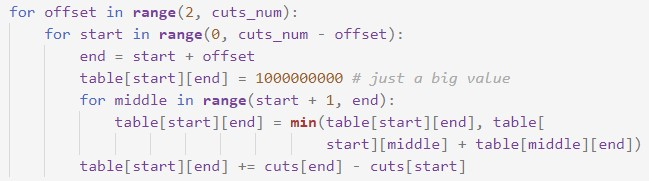
\includegraphics[width=5.2in]{algorithm.jpg}
        \end{center}
    \end{description}
\end{enumerate}

\end{document} 
